\lecture{Teoria delle Code}{22~-~01~-~2026}
%
%
\section{Definizione}
Una coda è un sistema rappresentato essenzialmente da quattro elementi costitutivi:
\begin{enumerate}
    \item Processo degli arrivi: Il modello che descrive come gli utenti o i job arrivano al sistema (può essere deterministico o stocastico, con arrivi singoli o a gruppi);
    \item Parametri strutturali: Le caratteristiche fisiche del sistema, quali il numero di posti nel buffer e il numero di serventi;
    \item Processo di uscita: Il modello che descrive il completamento del servizio (anche questo deterministico o stocastico);
    \item Disciplina della coda: La regola con cui vengono serviti gli utenti; in questo contesto l'analisi si focalizza sulla disciplina FIFO (\emph{First In, First Out}).
\end{enumerate}
Vedi figura \ref{fig:code1} a riguardo.
\begin{figure}
    \centering
    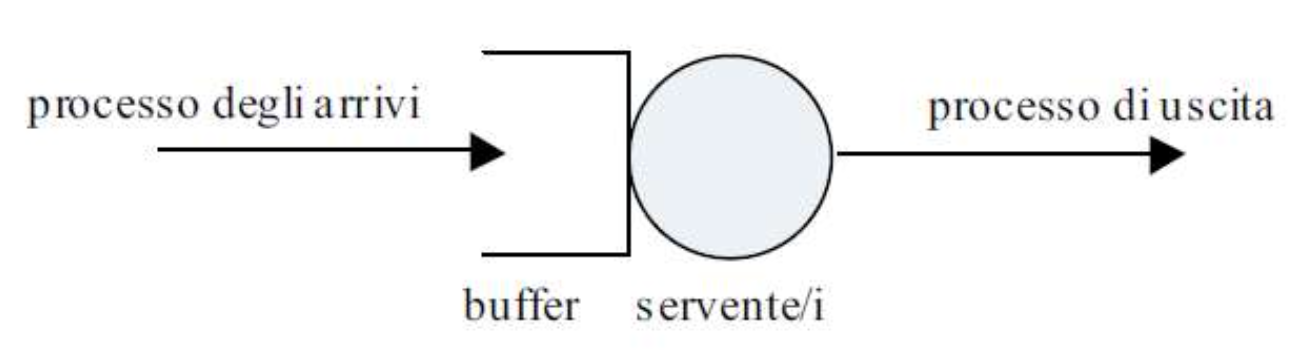
\includegraphics[width=0.5\linewidth]{assets/Screenshot 2026-01-22 at 16.27.36.png}
    \caption{Struttura di una coda.}\label{fig:code1}
\end{figure}

%
\subsection{Notazione di Kendall}
Per descrivere sinteticamente le code FIFO con arrivi singoli, si utilizza la notazione standard di Kendall composta da quattro elementi:
\[
    X_{a}/X_{s}/x_{ns}/x_{cap}
\]
\begin{itemize}
    \item $ X_{a} $ \textbf{(Tempi di arrivo)}: M (Markoviano (Processo di Poisson)), D (Deterministico), G (Generico stocastico);
    \item $ X_{s} $ \textbf{(Tempi di servizio)}: Utilizza le stesse sigle (M, D, G) per descrivere la distribuzione della durata del servizio;
    \item $ x_{ns} $: Indica il numero di serventi attivi;
    \item $ x_{cap} $: Rappresenta la capacità complessiva della risorsa (somma di buffer e serventi). Se la capacità è infinita ($\infty$), questo parametro viene omesso.
\end{itemize}
\begin{example}
    Alcuni esempi includono: $ M/D/2/4 $, la classica $ M/M/1 $, $ G/M/5 $, $ D/D/4/4 $ \dots
\end{example}
%
\section{Indice di prestazione e Legge di Little}
Per valutare l'efficienza di una coda, si monitorano specifici indici prestazionali:
\begin{enumerate}[label=\roman*)] % % chktex-file 9 % chktex-file 10
    \item $N$ e $L$: Numero medio di clienti rispettivamente nel sistema ($N$) e nella sola coda ($L$);
    \item Intensità di traffico ($\rho$, \emph{rho}): Il rapporto tra il tasso medio degli arrivi e il tasso di servizio;
    \item Fattore di utilizzo ($\eta$, \emph{eta}): La frazione di tempo in cui il servente è occupato;
    \item Throughput ($\gamma$, \emph{gamma}): Il numero di clienti serviti per unità di tempo;
    \item $S$ e $W$: Tempo medio di attraversamento totale del sistema ($S$) e tempo medio di attesa in coda ($W$);
\end{enumerate}

%
\paragraph{Legge di Little} È fondamentale per lo studio dei sistemi a regime stazionario, stabilisce che il numero medio di clienti nel sistema è il prodotto tra il tasso di entrata e il tempo di attraversamento: % chktex-file 17
\[
    N = \lambda_{in} S
\]
Analogalmente, per la coda:
\[
    L = \lambda_{in} W
\]
Vedi figura \ref{fig:little} per una rappresentazione grafica.
\begin{note*}
    Se il buffer è finito, il tasso di entrata $\lambda_{in}$ potrebbe essere inferiore al tasso di arrivo effettivo, poiché alcuni elementi vengono scartati e non entrano nella coda.
\end{note*}
\begin{figure}
    \centering
    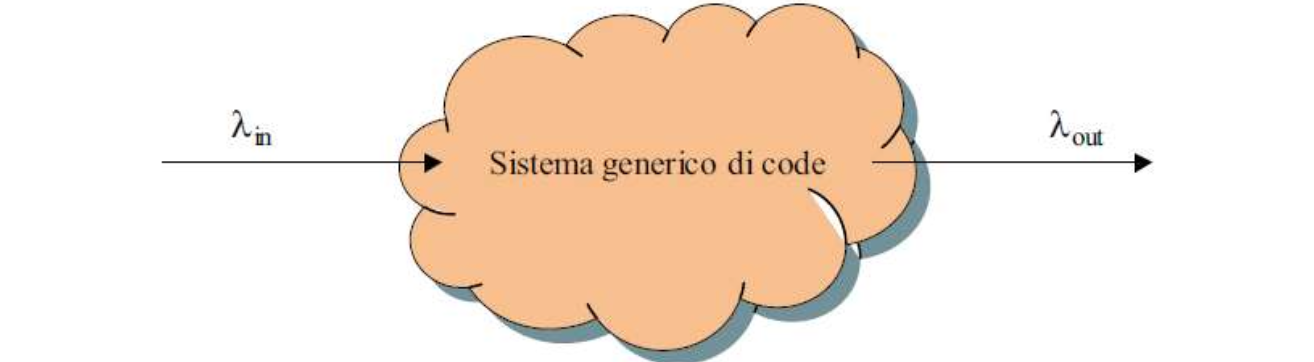
\includegraphics[width=0.7\linewidth]{assets/Screenshot 2026-01-22 at 16.57.39.png}
    \caption{Legge di Little}\label{fig:little}
\end{figure}

%
\section{Coda Markoviana M/M/1}
La coda M/M/1 è il modello base: markoviana, ergodica, con un solo operatore e buffer infinito. L'intensità di traffico è definita come:
\[
    \rho=\frac{\lambda}{\mu}
\]
Affinché il sistema sia stabile, è necessario che $\rho < 1$, ovvero che il tasso di arrivo sia inferiore al tasso di servizio.

Se $ \rho<1 $, e quindi il sistema è stabile, allora valgono le seguenti relazioni:
\begin{itemize}
    \item Probabilità di avere $k$ clienti: $\pi_{k} = (1-\rho)\rho^{k}$;
    \item Fattore di utilizzo: $\eta = \rho$;
    \item Numero medio clienti nel sistema: $N = \frac{\rho}{1-\rho}$;
    \item Tempo medio di attraversamento: $S = \frac{1}{\mu - \lambda}$;
    \item Tempo medio di attesa in coda: $W = \frac{\rho}{\mu(1-\rho)}$;
    \item Numero medio clienti in coda: $L = \frac{\rho^2}{1-\rho}$;
    \item Il throughput $\gamma$ in una coda stabile coincide con il tasso di arrivo $\lambda$.
\end{itemize}

%
\section{Coda M/M/m multi-servente}
In questo scenario, pur mantenendo un processo di nascita e morte, gli stati variano in base al numero di serventi $m$. Il tasso di servizio cambia dinamicamente: diventa $n\mu$ quando ci sono $n < m$ utenti, e si stabilizza a $m\mu$ quando ci sono $m$ o più utenti.
\begin{figure}
    \centering
    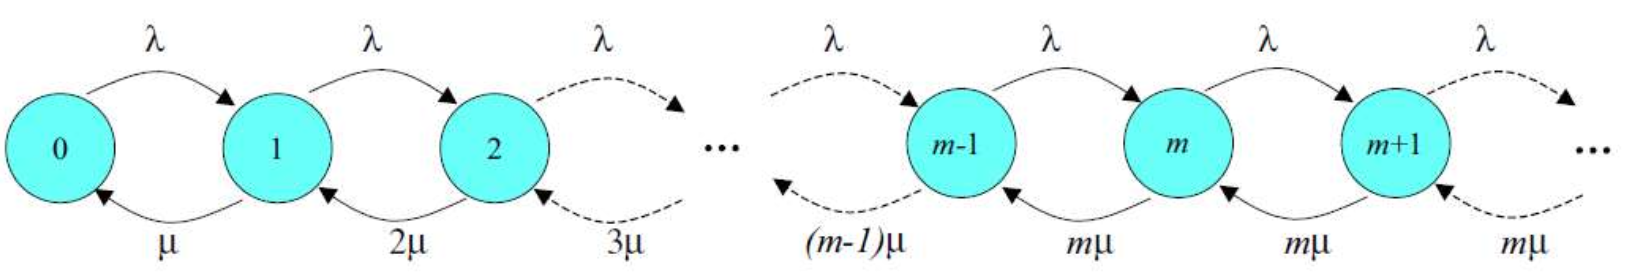
\includegraphics[width=1\linewidth]{assets/Screenshot 2026-01-22 at 17.05.49.png}
    \caption{Coda multi-servente M/M/m}\label{fig:mmm}
\end{figure}
Per una coda M/M/2 valgono le seguenti relazioni:
\begin{itemize}
    \item $\pi_0 = \frac{1-\rho}{1+\rho}$;
    \item $N = \frac{2\rho}{1-\rho^2}$;
    \item $S = \frac{1}{\mu(1-\rho^2)}$
\end{itemize}
Per sistemi più complessi, il calcolo analitico diventa oneroso e si preferisce spesso la simulazione al computer. Vedi figura \ref{fig:mmm} per un esempio di coda M/M/m.

%
\section{Reti di code aperte}
Le reti di code aperte sono sistemi composti da più stazioni $M/M/m$ collegate tra loro con routing probabilistico.
%
\paragraph{Condizioni di Stabilità} L'intera rete è considerata ergodica se e solo se tutte le singole risorse che la compongono sono stabili, ovvero se per ogni nodo vale:
\[
    \frac{\lambda}{\mu} < m
\]
%
\paragraph{Teorema di Burke, Proprietà dei Flussi} Due principi cardine permettono di analizzare queste reti sono il teorema di Burke e la Proprietà dei Flussi:
\begin{enumerate}
    \item L'uscita di una coda $M/M/m$ ergodica con tasso di arrivo $\lambda$ è un processo di Poisson con il medesimo tasso $\lambda$;
    \item Le operazioni di unione (merge) o divisione (split) di flussi di Poisson tramite routing probabilistico preservano la natura poissoniana dei flussi stessi.
\end{enumerate}
%
\paragraph{Risoluzione di reti con feedback (loop)} In presenza di un loop dove una frazione $p$ del flusso ritorna in coda (es. rilavorazione), il tasso di arrivo effettivo $\lambda$ alla risorsa aumenta rispetto al tasso di ingresso esterno $\gamma$. La relazione è data da:
\[
    \lambda = \gamma + p\lambda \quad \Rightarrow \quad \lambda = \frac{1}{1-p}\gamma
\]
Di conseguenza, l'intensità di traffico ricalcolata diventa:
\[
    \rho= \frac{\lambda}{\mu} = \frac{1}{1-p} \frac{\gamma}{\mu}
\]
Infine, se $ \rho<1 $, la coda è ergodica, e calcoliamo:
\[
    N=\frac{\rho}{1-\rho}, S=\frac{N}{\gamma}
\]
%
\paragraph{Calcolo dei Tempi Totali} Per calcolare il tempo totale di attraversamento di una rete, si calcola prima il numero medio di utenti $N_i$ per ogni singola coda, poi si applica la legge di Little complessiva:
\[
    S_{tot} = \frac{\sum{N_{i}}}{\lambda_{ingresso}}
\]
\begin{example}
    Avendo due code in serie, Il processo in uscita dalla prima
    coda è Poisson con tasso $\lambda$ (Burke).

    Se $ \rho_{1},\rho_{2}<1 $ allora la coda è ergodica e usiamo la legge di Little per calcolare il tempo totale di attraversamento della rete di code:
    \[
        S = \frac{N_{1}+N_{2}}{\lambda}
    \]
    Vedi figura \ref{fig:ex1} riguardo l'esempio e le formule di $ \rho_{n} $ e $ N_{n} $
    \begin{figure}
        \centering
        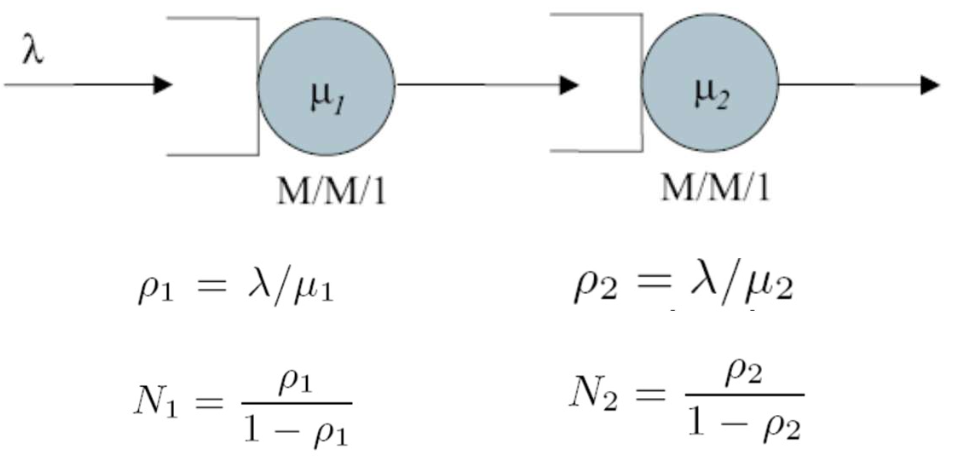
\includegraphics[width=0.5\linewidth]{assets/Screenshot 2026-01-22 at 17.24.10.png}
        \caption{Esempio di rete di code in serie.}\label{fig:ex1}
    \end{figure}
\end{example}